% This file was converted to LaTeX by Writer2LaTeX ver. 1.0.2
% see http://writer2latex.sourceforge.net for more info
\documentclass{article}
\usepackage[utf8]{inputenc}
\usepackage[T1]{fontenc}
\usepackage[french]{babel}
\usepackage{amsmath}
\usepackage{amssymb,amsfonts,textcomp}
\usepackage{array}
\usepackage{supertabular}
\usepackage{hhline}
\usepackage[pdftex]{graphicx}
\makeatletter
\newcommand\arraybslash{\let\\\@arraycr}
\makeatother
\setlength\tabcolsep{1mm}
\renewcommand\arraystretch{1.3}
\title{}
\author{}
\date{}
\begin{document}
\section[BEST PRACTICE N°1]{BEST PRACTICE N°1}
\subsection[Aide à la rédaction d’une procédure]{Aide à la rédaction
d’une procédure}

\bigskip


\bigskip

Objectif de ce document : Définir les règles de rédaction d’une
procédure devant intégrer le système documentaire dans le cadre du
projet COPEVUE-MONIT


\bigskip

\subsubsection[1. Définitions]{1. Définitions}
Procédure : Manière spécifiée d’accomplir une activité

(Cf. ISO 8402)


\bigskip

Une procédure écrite comporte généralement :

\begin{itemize}
\item l’objet et  le domaine d’application
\item ce qui doit être fait et qui doit le faire : QUI ?
\item ou et quand cela doit être fait : OU ? QUAND ?
\item les moyens qui doivent être utilisés : QUOI ?
\item comment cela doit  être maîtrisé et  enregistré : COMMENT ?
\end{itemize}

\bigskip

\subsubsection[2. Documents de référence]{2. Documents de référence}

\bigskip

GLOSSAIRE / Glossaire qualité

QUALITE / Gestion de la documentation


\bigskip

\subsubsection[3. Méthodologie de rédaction]{3. Méthodologie de
rédaction}
\paragraph[3.1. Mise en oeuvre du QQOQCP]{3.1. Mise en oeuvre du QQOQCP}
Une procédure est un document décrivant une activité spécifique
(COMMENT?) du système concerné en précisant les responsabilités (QUI ?
OU? QUAND?)  les interactions entre les services et les moyens (QUOI?)
requis pour obtenir le résultat prévu (POURQUOI?)


\bigskip

 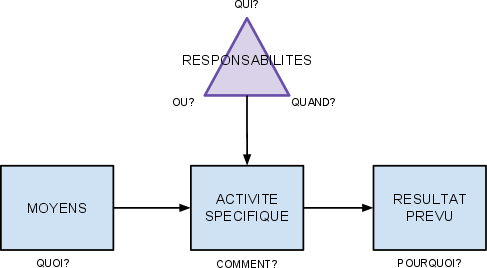
\includegraphics[width=12.885cm,height=7.673cm]{BP1-img1.png} 

\paragraph[3.2. Méthode pour rédiger une procédure]{3.2. Méthode pour
rédiger une procédure}

\bigskip

\subparagraph[LOGIGRAMME DE RÉDACTION D’UNE PROCÉDURE :]{LOGIGRAMME DE
RÉDACTION D’UNE PROCÉDURE :}

\bigskip

 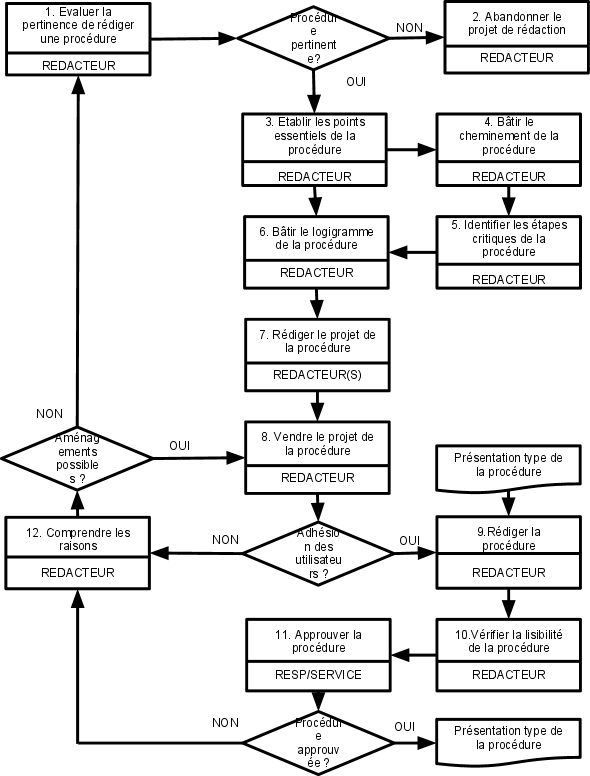
\includegraphics[width=15.637cm,height=20.535cm]{BP1-img2.png} 

\subsubsection[4. Contenu d’une procédure]{4. Contenu d’une procédure}
\paragraph[4.1. Présentation]{4.1. Présentation}

\bigskip

Le document de type
{\textless}{\textless}Procédure{\textgreater}{\textgreater} doit
respecter les éléments de structure et de présentation énoncés dans le
dossier QUALITE / Gestion de la documentation :


\bigskip

\begin{flushleft}
\tablehead{}
\begin{supertabular}{|m{16.345cm}|}
\hline
Il est convenu que tout document doit comporter les éléments suivants
sur la page de garde :

\begin{itemize}
\item le titre du document,\item la référence du document,\item la date
de dernière mise à jour,\item le nom de l’auteur (ou des auteurs),\item
l’objet du document (présentation rapide du contenu)\end{itemize}
~

D’autre part, sur chaque page du document préciser :

\begin{itemize}
\item le titre du document,\item la référence,\item le numéro de page /
nombre de pages total.\end{itemize}
\\\hline
\end{supertabular}
\end{flushleft}

\bigskip

\paragraph[4.2. Objet]{4.2. Objet}

\bigskip

Avant tout il est important de pouvoir définir l’objet de la procédure :
il faut pouvoir expliquer la raison d’être du document, ainsi que les
objectifs qu’elle permet d’atteindre.


\bigskip

\paragraph[4.3. Domaine d’application]{4.3. Domaine d’application}

\bigskip

Il s’agit ici de définir le périmètre couvert par la procédure en
précisant les entrées et sorties identifiées du processus qu’elle
décrit et de décliner sa place dans le système documentaire qualité en
précisant ses attachements aux autres documents


\bigskip

\paragraph[4.4. Plan type]{4.4. Plan type}

\bigskip

1. Objet

2. Documents de référence

3. Domaine d’application

4. Logigramme de la procédure

5. Tableau de définition des actions

6. Outils nécessaires

(7. Exemples)


\bigskip

\paragraph[4.5. Description des parties à rédiger]{4.5. Description des
parties à rédiger}
\subparagraph[4.5.1. Objet]{4.5.1. Objet}
Cette section rappelle les raisons du pourquoi de la procédure
(généralement, les raisons concernant des exigences requises et les
méthodes à mettre en oeuvre pour maîtriser un processus)

\subparagraph[4.5.2. Documents de référence]{4.5.2. Documents de
référence}
Documents nécessaires à la bonne compréhension du document dans son
intégralité. Par exemple, référence vers d’autres procédures.

\subparagraph[4.5.3. Domaine d’application]{4.5.3. Domaine
d’application}
Cette rubrique indique qui, dans l’organisation, est concerné par cette
procédure. Délimite également le périmètre couvert par la procédure

\subparagraph[4.5.4. Logigramme de la procédure]{4.5.4. Logigramme de la
procédure}
Le déroulement du processus doit être décrit sous la forme d’un
logigramme simple mais complet. 


\bigskip

Un logigramme doit comporter les éléments suivants :


\bigskip

\begin{flushleft}
\tablehead{}
\begin{supertabular}{|m{5.727cm}|m{10.419001cm}|}
\hline
\centering FORME &
\centering\arraybslash DESCRIPTION\\\hline
\centering  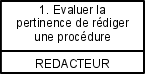
\includegraphics[width=3.863cm,height=1.958cm]{BP1-img3.png}
 &
ACTION définissant une activité. Doit comporter :

\begin{itemize}
\item Le numéro de l’action\item Le titre de l’action (description
courte)\item L’auteur de l’action\end{itemize}
\\\hline
\centering  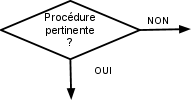
\includegraphics[width=5.054cm,height=2.672cm]{BP1-img4.png}
 &
QUESTION impliquant un choix ou une différente possibilité. Chaque
sortie représente une possibilité de réponse à la question
posée.\\\hline
\centering  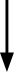
\includegraphics[width=0.529cm,height=1.905cm]{BP1-img5.png}
 &
LIAISON indiquant un flux, une transition entre deux actions. Implique
une transformation d’une sortie vers une nouvelle entrée.\\\hline
\centering  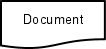
\includegraphics[width=2.805cm,height=1.323cm]{BP1-img6.png}
 &
DOCUMENT utilisé par une action ou une activité. On suppose que le
document a déjà été rédigé.\\\hline
\end{supertabular}
\end{flushleft}

\bigskip

Afin de retrouver un exemple de logigramme, vous pouvez vous référer à
celui présent dans ce document même, dans la section 3.2. Méthode pour
rédiger une procédure.


\bigskip

\subparagraph[4.5.5. Tableau de définition des actions]{4.5.5. Tableau
de définition des actions}
Pour chaque action identifiée dans le logigramme, nous allons les
décrire plus précisément afin d’identifier très clairement l’activité
concernée.\newline
Pour celà, nous utiliserons un tableau des actions, récapitulant le
numéro de l’action, son intitulé, sa description complète ainsi que les
documents impliqués dans l’élaboration de l’activité.


\bigskip

Un tel tableau se présente sous la forme :

\begin{flushleft}
\tablehead{}
\begin{supertabular}{|m{1.4139999cm}|m{3.24cm}|m{8.293cm}|m{2.799cm}|}
\hline
\centering Action &
\centering Intitulé &
\centering Description &
\centering\arraybslash Documents impliqués\\\hline
\centering 1 &
Nom de l’action 1 &
Description complète de l’action : description des différentes
sous-étapes nécessaires à la réalisation de l’action. (4 à 5 lignes) &
Document de référence 1\\\hline
\centering 2 &
Nom de l’action 2 &
... &
Document 2\\\hline
\centering 3 &
... &
... &
...\\\hline
\end{supertabular}
\end{flushleft}

\bigskip

\subparagraph[4.5.6. Outils nécessaires]{4.5.6. Outils nécessaires}
Liste des outils nécessaires afin d’effectuer la procédure. Dans cette
partie, le rédacteur peut présenter les différents outils qu’il
recommande d’utiliser afin de compléter la procédure dans son
intégralité. On peut par exemple citer des modèles de documents
particuliers, des feuilles de calculs à réutiliser, des progiciels
permettant de simplifier le travail à réaliser.

Si l’on désire en savoir plus sur l’installation ou l’utilisation de ces
outils, on pourra les présenter plus en détail en annexe de la
procédure.

\subparagraph[4.5.7. Exemples]{4.5.7. Exemples}
Si la procédure mérite une illustration, il est possible de présenter un
exemple présentant le résultat final d’un document respectant les
différentes étapes de la procédure.

\subsubsection[5. Gestion du document]{5. Gestion du document}

\bigskip

Le document de type
{\textless}{\textless}Procédure{\textgreater}{\textgreater} doit
respecter les éléments de gestion de la documentation énoncés dans le
dossier QUALITE / Gestion de la documentation.
\end{document}
